\documentclass[twocolumn,a4j]{jsarticle}
\setlength{\topmargin}{-20.4cm}
\setlength{\oddsidemargin}{-10.4mm}
\setlength{\evensidemargin}{-10.4mm}
\setlength{\textwidth}{18cm}
\setlength{\textheight}{26cm}

\usepackage[top=15truemm,bottom=20truemm,left=20truemm,right=20truemm]{geometry}
\usepackage[latin1]{inputenc}
\usepackage{amsmath}
\usepackage{amsfonts}
\usepackage{amssymb}
\usepackage[dvipdfmx]{graphicx}
\usepackage[hang,small,bf]{caption}
\usepackage[subrefformat=parens]{subcaption}
\usepackage[dvipdfmx]{color}
\usepackage{listings}
\usepackage{listings,jvlisting}
\usepackage{geometry}
\usepackage{framed}
\usepackage{color}
\usepackage[dvipdfmx]{hyperref}
\usepackage{ascmac}
\usepackage{enumerate}
\usepackage{tabularx}
\usepackage{cancel}
\usepackage{scalefnt}
\usepackage{overcite}
\usepackage{otf}
\usepackage{multicol}
\usepackage[geometry]{ifsym}
\usepackage{array}

\renewcommand{\figurename}{Fig.}
\renewcommand{\tablename}{Table }

\lstset{
basicstyle={\ttfamily},
identifierstyle={\small},
commentstyle={\smallitshape},
keywordstyle={\small\bfseries},
ndkeywordstyle={\small},
stringstyle={\small\ttfamily},
frame={tb},
breaklines=true,
columns=[l]{fullflexible},
xrightmargin=0zw,
xleftmargin=3zw,
numberstyle={\scriptsize},
stepnumber=1,
numbersep=1zw,
lineskip=-0.5ex
}

% キャプション後ろのダブルコロンを消す
\makeatletter
\long\def\@makecaption#1#2{%
  \vskip\abovecaptionskip
  \iftdir\sbox\@tempboxa{#1\hskip1zw#2}%
    \else\sbox\@tempboxa{#1 #2}%
  \fi
  \ifdim \wd\@tempboxa >\hsize
    \iftdir #1\hskip1zw#2\relax\par
      \else #1 #2\relax\par\fi
  \else
    \global \@minipagefalse
    \hbox to\hsize{\hfil\box\@tempboxa\hfil}%
  \fi
  \vskip\belowcaptionskip}
\makeatother

% タイトル
\makeatletter
\def\@maketitle
{
\begin{center}
{\LARGE \@title \par}
\end{center}
\begin{flushright}
{\large \@date 報告書 No.34}\\
{\large M2 \@author}
\end{flushright}
\par\vskip 1.5em
}
\makeatother

\author{来代 勝胤}
\title{令和4年度 9月 第1週 報告書}
\date{2022/9/5}

\begin{document}
\columnseprule=0.1mm
\maketitle

\section*{報告内容}
\begin{enumerate}[1.]
  \item 解析アルゴリズムの再構成
  \item 来週の予定
\end{enumerate}

\section{解析アルゴリズムの再構成}
\begin{enumerate}[(1)]
  \item [] \textgt{[ 全体の流れ ]}
  \item 校正ブロックの校正点特定と補正関数の取得
  \item 背景処理・粒子位置特定等の前処理
  \item 粒子追跡
  \item ベクトルの再配置・誤ベクトル除去等の後処理
\end{enumerate}

\subsection{(3) 粒子追跡について}

\subsection*{粒子像の特徴 [1] : 粒子位置のスライド}
以下のFig.1は,各色の粒子像について,時刻ごとの粒子の移動を示している.
総じて,時刻経過による移動量は非常に小さく,
傾向として時刻経過にしたがって右に移動していくことがわかる.
したがって,同一粒子の判定に用いる粒子追跡手法は最近法を用いて追跡が可能だと考えられる.

\begin{figure}[htbp]
  \begin{tabular}{cc}
    \begin{minipage}[t]{0.45\hsize}
      \centering
      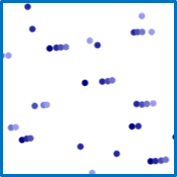
\includegraphics[keepaspectratio, width=35mm]{../images/time-line_blue.png}
      \subcaption{Blue}
    \end{minipage} &
    \begin{minipage}[t]{0.45\hsize}
      \centering
      
\includegraphics[keepaspectratio, width=35mm]{../images/time-line_green.png}
      \subcaption{Green}
    \end{minipage}
  \end{tabular}
  \caption{Particle Timeline}
  \centering ※色が濃い点ほど時刻が若い
\end{figure}

\subsection*{粒子像の特徴 [1] : 二次流れの解析}
次に,Fig.2 に青の緑の粒子像を重ね合わせた例を示す.
この画像からも,最近法によって
粒子を追跡することが可能であると考えられる.

\begin{figure}[htbp]
  \centering
  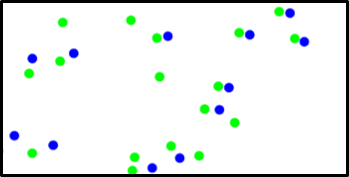
\includegraphics[keepaspectratio, width=60mm]{../images/merged_particles.png}
  \caption{Overlap particles}
\end{figure}

\newpage
\subsection*{粒子追跡手順}
\begin{itemize}
  \item 最近法による追跡
  \item 誤ベクトル除去
\end{itemize}

\subsection*{誤ベクトル処理の手順}
\begin{itemize}
  \item 上位と下位 10\% の大きさを持つベクトルデータを除いたデータを作成.(トリムデータの作成)
  \item トリムデータから平均値と標準偏差を計算
  \item 平均値 + 2倍の標準偏差 を超えるベクトルを除去する
\end{itemize}

\begin{figure}[htbp]
  \begin{tabular}{cc}
    \begin{minipage}[t]{0.45\hsize}
      \centering
      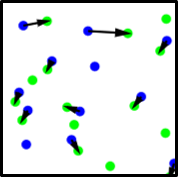
\includegraphics[keepaspectratio, width=35mm]{../images/vector_before.png}
      \subcaption{Before}
    \end{minipage} &
    \begin{minipage}[t]{0.45\hsize}
      \centering
      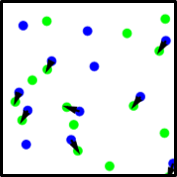
\includegraphics[keepaspectratio, width=35mm]{../images/vector_after.png}
      \subcaption{After}
    \end{minipage}
  \end{tabular}
  \caption{Erroneous vector removal}
\end{figure}

\section{来週の予定}
\begin{itemize}
  \item 解析アルゴリズムの再構成 (続)
  \item ISTP スライド作成
\end{itemize}

\end{document}